\section{Methodology}

\subsection{Test Environment}
\begin{table}
    \begin{tabular}{l|l}
        \hline
        \hline
    Manufacturer    & Hardkernel\\
    Platform        & Odroid-X2\\
    SoC             & Samsung Exynos 4412 "Prime"\\
    CPU Core        & ARM Cortex-A9\\
    Number of cores & 4\\
    Clock Freq.     & 1.7GHz\\
    Core Voltage    & 1.3V\\
    OS              & Debian testing ``jessie''\\
    Kernel          & 3.8 custom\\
        \hline
        \hline
    Voltmeter       & Agilent 34410A\\
    Power supply    & Agilent E3631A\\
    Shunt resistor  & 12m$\Omega$\\
        \hline
        \hline
    \end{tabular}
    \caption{System specifications}
    \label{table:system_spec}
\end{table}

In our experiments, we are using the ODROID-X2 \cite{odroid-x2} developer
platform, which has an Exynos 4412 "Prime" System-on-Chip with four ARM
Cortex-A9 (r3p0) processor cores. We disable three of the cores, leaving only
one core configured to run at a fixed frequency of $1.7$ GHz. The test
environment is sketched in \ref{fig:setup}, while the details are summarized in
\ref{table:system_spec}.

\begin{figure}
    % Graphic for TeX using PGF
% Title: /backup/hvatum/Skole/arm-project/report/figures/test_setup.xml
% Creator: Dia v0.97.2
% CreationDate: Wed Dec 11 22:34:20 2013
% For: hvatum
% \usepackage{tikz}
% The following commands are not supported in PSTricks at present
% We define them conditionally, so when they are implemented,
% this pgf file will use them.
\ifx\du\undefined
  \newlength{\du}
\fi
\setlength{\du}{15\unitlength}
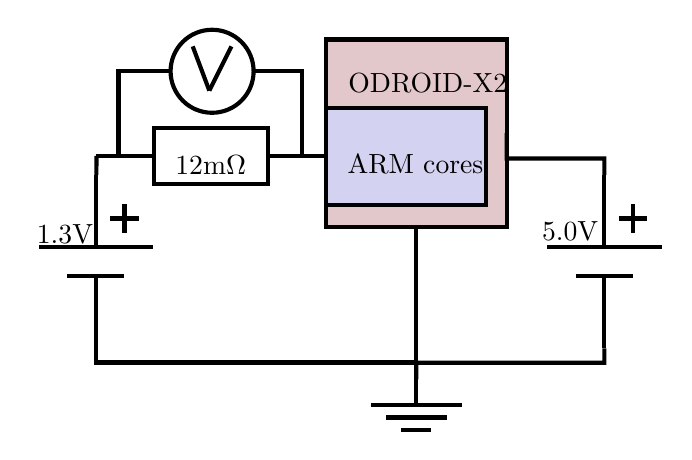
\begin{tikzpicture}
\pgftransformxscale{1.000000}
\pgftransformyscale{-1.000000}
\definecolor{dialinecolor}{rgb}{0.000000, 0.000000, 0.000000}
\pgfsetstrokecolor{dialinecolor}
\definecolor{dialinecolor}{rgb}{1.000000, 1.000000, 1.000000}
\pgfsetfillcolor{dialinecolor}
\pgfsetlinewidth{0.100000\du}
\pgfsetdash{}{0pt}
\pgfsetdash{}{0pt}
\pgfsetbuttcap
\pgfsetmiterjoin
\pgfsetlinewidth{0.100000\du}
\pgfsetbuttcap
\pgfsetmiterjoin
\pgfsetdash{}{0pt}
\definecolor{dialinecolor}{rgb}{0.000000, 0.000000, 0.000000}
\pgfsetstrokecolor{dialinecolor}
\draw (19.962100\du,12.768751\du)--(21.337939\du,12.768751\du);
\pgfsetbuttcap
\pgfsetmiterjoin
\pgfsetdash{}{0pt}
\definecolor{dialinecolor}{rgb}{1.000000, 1.000000, 1.000000}
\pgfsetfillcolor{dialinecolor}
\fill (21.337939\du,12.097000\du)--(21.337939\du,13.440503\du)--(24.089616\du,13.440503\du)--(24.089616\du,12.097000\du)--cycle;
\definecolor{dialinecolor}{rgb}{0.000000, 0.000000, 0.000000}
\pgfsetstrokecolor{dialinecolor}
\draw (21.337939\du,12.097000\du)--(21.337939\du,13.440503\du)--(24.089616\du,13.440503\du)--(24.089616\du,12.097000\du)--cycle;
\pgfsetbuttcap
\pgfsetmiterjoin
\pgfsetdash{}{0pt}
\definecolor{dialinecolor}{rgb}{0.000000, 0.000000, 0.000000}
\pgfsetstrokecolor{dialinecolor}
\draw (24.089616\du,12.768751\du)--(25.465455\du,12.768751\du);
% setfont left to latex
\definecolor{dialinecolor}{rgb}{0.000000, 0.000000, 0.000000}
\pgfsetstrokecolor{dialinecolor}
\node[anchor=west] at (18.254748\du,14.648958\du){1.3V};
% setfont left to latex
\definecolor{dialinecolor}{rgb}{0.000000, 0.000000, 0.000000}
\pgfsetstrokecolor{dialinecolor}
\node[anchor=west] at (18.254748\du,15.448958\du){};
\pgfsetlinewidth{0.100000\du}
\pgfsetdash{}{0pt}
\pgfsetdash{}{0pt}
\pgfsetbuttcap
\pgfsetmiterjoin
\pgfsetlinewidth{0.100000\du}
\pgfsetbuttcap
\pgfsetmiterjoin
\pgfsetdash{}{0pt}
\definecolor{dialinecolor}{rgb}{0.890196, 0.784314, 0.796078}
\pgfsetfillcolor{dialinecolor}
\fill (25.484300\du,9.968170\du)--(25.484300\du,14.476173\du)--(29.846883\du,14.476173\du)--(29.846883\du,9.968170\du)--cycle;
\definecolor{dialinecolor}{rgb}{0.000000, 0.000000, 0.000000}
\pgfsetstrokecolor{dialinecolor}
\draw (25.484300\du,9.968170\du)--(25.484300\du,14.476173\du)--(29.846883\du,14.476173\du)--(29.846883\du,9.968170\du)--cycle;
\pgfsetbuttcap
\pgfsetmiterjoin
\pgfsetdash{}{0pt}
\definecolor{dialinecolor}{rgb}{0.000000, 0.000000, 0.000000}
\pgfsetstrokecolor{dialinecolor}
\draw (25.484300\du,9.968170\du)--(25.484300\du,14.476173\du)--(29.846883\du,14.476173\du)--(29.846883\du,9.968170\du)--cycle;
% setfont left to latex
\definecolor{dialinecolor}{rgb}{0.000000, 0.000000, 0.000000}
\pgfsetstrokecolor{dialinecolor}
\node[anchor=west] at (25.759875\du,11.008700\du){ODROID-X2};
\pgfsetlinewidth{0.100000\du}
\pgfsetdash{}{0pt}
\pgfsetdash{}{0pt}
\pgfsetmiterjoin
\definecolor{dialinecolor}{rgb}{0.827451, 0.823529, 0.941176}
\pgfsetfillcolor{dialinecolor}
\fill (25.486700\du,11.611400\du)--(25.486700\du,13.961400\du)--(29.337189\du,13.961400\du)--(29.337189\du,11.611400\du)--cycle;
\definecolor{dialinecolor}{rgb}{0.000000, 0.000000, 0.000000}
\pgfsetstrokecolor{dialinecolor}
\draw (25.486700\du,11.611400\du)--(25.486700\du,13.961400\du)--(29.337189\du,13.961400\du)--(29.337189\du,11.611400\du)--cycle;
% setfont left to latex
\definecolor{dialinecolor}{rgb}{0.000000, 0.000000, 0.000000}
\pgfsetstrokecolor{dialinecolor}
\node[anchor=west] at (25.737200\du,12.964800\du){ARM cores};
% setfont left to latex
\definecolor{dialinecolor}{rgb}{0.000000, 0.000000, 0.000000}
\pgfsetstrokecolor{dialinecolor}
\node[anchor=west] at (30.423200\du,14.580700\du){5.0V};
\pgfsetlinewidth{0.100000\du}
\pgfsetdash{}{0pt}
\pgfsetdash{}{0pt}
\pgfsetbuttcap
\pgfsetmiterjoin
\pgfsetlinewidth{0.100000\du}
\pgfsetbuttcap
\pgfsetmiterjoin
\pgfsetdash{}{0pt}
\definecolor{dialinecolor}{rgb}{0.000000, 0.000000, 0.000000}
\pgfsetstrokecolor{dialinecolor}
\draw (27.667052\du,18.153700\du)--(27.667052\du,18.766668\du);
\pgfsetbuttcap
\pgfsetmiterjoin
\pgfsetdash{}{0pt}
\definecolor{dialinecolor}{rgb}{0.000000, 0.000000, 0.000000}
\pgfsetstrokecolor{dialinecolor}
\draw (26.568500\du,18.766668\du)--(28.765605\du,18.766668\du);
\pgfsetbuttcap
\pgfsetmiterjoin
\pgfsetdash{}{0pt}
\definecolor{dialinecolor}{rgb}{0.000000, 0.000000, 0.000000}
\pgfsetstrokecolor{dialinecolor}
\draw (26.936515\du,19.073151\du)--(28.397590\du,19.073151\du);
\pgfsetbuttcap
\pgfsetmiterjoin
\pgfsetdash{}{0pt}
\definecolor{dialinecolor}{rgb}{0.000000, 0.000000, 0.000000}
\pgfsetstrokecolor{dialinecolor}
\draw (27.304530\du,19.379635\du)--(28.029575\du,19.379635\du);
% setfont left to latex
\definecolor{dialinecolor}{rgb}{0.000000, 0.000000, 0.000000}
\pgfsetstrokecolor{dialinecolor}
\node at (22.713800\du,12.990050\du){12m$\Omega$};
\pgfsetlinewidth{0.100000\du}
\pgfsetdash{}{0pt}
\pgfsetdash{}{0pt}
\pgfsetbuttcap
\pgfsetmiterjoin
\pgfsetlinewidth{0.100000\du}
\pgfsetbuttcap
\pgfsetmiterjoin
\pgfsetdash{}{0pt}
\definecolor{dialinecolor}{rgb}{1.000000, 1.000000, 1.000000}
\pgfsetfillcolor{dialinecolor}
\pgfpathellipse{\pgfpoint{22.747033\du}{10.732410\du}}{\pgfpoint{1.000000\du}{0\du}}{\pgfpoint{0\du}{1.000000\du}}
\pgfusepath{fill}
\definecolor{dialinecolor}{rgb}{0.000000, 0.000000, 0.000000}
\pgfsetstrokecolor{dialinecolor}
\pgfpathellipse{\pgfpoint{22.747033\du}{10.732410\du}}{\pgfpoint{1.000000\du}{0\du}}{\pgfpoint{0\du}{1.000000\du}}
\pgfusepath{stroke}
\pgfsetbuttcap
\pgfsetmiterjoin
\pgfsetdash{}{0pt}
\definecolor{dialinecolor}{rgb}{0.000000, 0.000000, 0.000000}
\pgfsetstrokecolor{dialinecolor}
\draw (22.680367\du,11.199077\du)--(23.213700\du,10.132410\du);
\pgfsetbuttcap
\pgfsetmiterjoin
\pgfsetdash{}{0pt}
\definecolor{dialinecolor}{rgb}{0.000000, 0.000000, 0.000000}
\pgfsetstrokecolor{dialinecolor}
\draw (22.680367\du,11.199077\du)--(22.280367\du,10.132410\du);
\pgfsetbuttcap
\pgfsetmiterjoin
\pgfsetdash{}{0pt}
\definecolor{dialinecolor}{rgb}{0.000000, 0.000000, 0.000000}
\pgfsetstrokecolor{dialinecolor}
\draw (20.613700\du,10.732410\du)--(21.747033\du,10.732410\du);
\pgfsetbuttcap
\pgfsetmiterjoin
\pgfsetdash{}{0pt}
\definecolor{dialinecolor}{rgb}{0.000000, 0.000000, 0.000000}
\pgfsetstrokecolor{dialinecolor}
\draw (23.747033\du,10.732410\du)--(24.880367\du,10.732410\du);
\pgfsetlinewidth{0.100000\du}
\pgfsetdash{}{0pt}
\pgfsetdash{}{0pt}
\pgfsetbuttcap
\pgfsetmiterjoin
\pgfsetlinewidth{0.100000\du}
\pgfsetbuttcap
\pgfsetmiterjoin
\pgfsetdash{}{0pt}
\definecolor{dialinecolor}{rgb}{0.000000, 0.000000, 0.000000}
\pgfsetstrokecolor{dialinecolor}
\draw (32.197597\du,13.236300\du)--(32.197597\du,14.973868\du);
\pgfsetbuttcap
\pgfsetmiterjoin
\pgfsetdash{}{0pt}
\definecolor{dialinecolor}{rgb}{0.000000, 0.000000, 0.000000}
\pgfsetstrokecolor{dialinecolor}
\draw (30.819800\du,14.973868\du)--(33.575394\du,14.973868\du);
\pgfsetbuttcap
\pgfsetmiterjoin
\pgfsetdash{}{0pt}
\definecolor{dialinecolor}{rgb}{0.000000, 0.000000, 0.000000}
\pgfsetstrokecolor{dialinecolor}
\draw (31.508699\du,15.668895\du)--(32.886496\du,15.668895\du);
\pgfsetbuttcap
\pgfsetmiterjoin
\pgfsetdash{}{0pt}
\definecolor{dialinecolor}{rgb}{0.000000, 0.000000, 0.000000}
\pgfsetstrokecolor{dialinecolor}
\draw (32.886496\du,13.931327\du)--(32.886496\du,14.626354\du);
\pgfsetbuttcap
\pgfsetmiterjoin
\pgfsetdash{}{0pt}
\definecolor{dialinecolor}{rgb}{0.000000, 0.000000, 0.000000}
\pgfsetstrokecolor{dialinecolor}
\draw (32.542046\du,14.278841\du)--(33.230945\du,14.278841\du);
\pgfsetbuttcap
\pgfsetmiterjoin
\pgfsetdash{}{0pt}
\definecolor{dialinecolor}{rgb}{0.000000, 0.000000, 0.000000}
\pgfsetstrokecolor{dialinecolor}
\draw (32.197597\du,15.668895\du)--(32.197597\du,17.406462\du);
\pgfsetlinewidth{0.100000\du}
\pgfsetdash{}{0pt}
\pgfsetdash{}{0pt}
\pgfsetbuttcap
\pgfsetmiterjoin
\pgfsetlinewidth{0.100000\du}
\pgfsetbuttcap
\pgfsetmiterjoin
\pgfsetdash{}{0pt}
\definecolor{dialinecolor}{rgb}{0.000000, 0.000000, 0.000000}
\pgfsetstrokecolor{dialinecolor}
\draw (19.947397\du,13.236300\du)--(19.947397\du,14.973868\du);
\pgfsetbuttcap
\pgfsetmiterjoin
\pgfsetdash{}{0pt}
\definecolor{dialinecolor}{rgb}{0.000000, 0.000000, 0.000000}
\pgfsetstrokecolor{dialinecolor}
\draw (18.569600\du,14.973868\du)--(21.325194\du,14.973868\du);
\pgfsetbuttcap
\pgfsetmiterjoin
\pgfsetdash{}{0pt}
\definecolor{dialinecolor}{rgb}{0.000000, 0.000000, 0.000000}
\pgfsetstrokecolor{dialinecolor}
\draw (19.258499\du,15.668895\du)--(20.636296\du,15.668895\du);
\pgfsetbuttcap
\pgfsetmiterjoin
\pgfsetdash{}{0pt}
\definecolor{dialinecolor}{rgb}{0.000000, 0.000000, 0.000000}
\pgfsetstrokecolor{dialinecolor}
\draw (20.636296\du,13.931327\du)--(20.636296\du,14.626354\du);
\pgfsetbuttcap
\pgfsetmiterjoin
\pgfsetdash{}{0pt}
\definecolor{dialinecolor}{rgb}{0.000000, 0.000000, 0.000000}
\pgfsetstrokecolor{dialinecolor}
\draw (20.291846\du,14.278841\du)--(20.980745\du,14.278841\du);
\pgfsetbuttcap
\pgfsetmiterjoin
\pgfsetdash{}{0pt}
\definecolor{dialinecolor}{rgb}{0.000000, 0.000000, 0.000000}
\pgfsetstrokecolor{dialinecolor}
\draw (19.947397\du,15.668895\du)--(19.947397\du,17.406462\du);
\pgfsetlinewidth{0.100000\du}
\pgfsetdash{}{0pt}
\pgfsetdash{}{0pt}
\pgfsetbuttcap
{
\definecolor{dialinecolor}{rgb}{0.000000, 0.000000, 0.000000}
\pgfsetfillcolor{dialinecolor}
% was here!!!
\definecolor{dialinecolor}{rgb}{0.000000, 0.000000, 0.000000}
\pgfsetstrokecolor{dialinecolor}
\draw (19.962100\du,12.768800\du)--(19.959407\du,13.236300\du);
}
\pgfsetlinewidth{0.100000\du}
\pgfsetdash{}{0pt}
\pgfsetdash{}{0pt}
\pgfsetmiterjoin
\pgfsetbuttcap
{
\definecolor{dialinecolor}{rgb}{0.000000, 0.000000, 0.000000}
\pgfsetfillcolor{dialinecolor}
% was here!!!
{\pgfsetcornersarced{\pgfpoint{0.000000\du}{0.000000\du}}\definecolor{dialinecolor}{rgb}{0.000000, 0.000000, 0.000000}
\pgfsetstrokecolor{dialinecolor}
\draw (29.846900\du,12.222200\du)--(29.846900\du,12.833100\du)--(32.197516\du,12.833100\du)--(32.197529\du,13.236170\du);
}}
\pgfsetlinewidth{0.100000\du}
\pgfsetdash{}{0pt}
\pgfsetdash{}{0pt}
\pgfsetmiterjoin
\pgfsetbuttcap
{
\definecolor{dialinecolor}{rgb}{0.000000, 0.000000, 0.000000}
\pgfsetfillcolor{dialinecolor}
% was here!!!
{\pgfsetcornersarced{\pgfpoint{0.000000\du}{0.000000\du}}\definecolor{dialinecolor}{rgb}{0.000000, 0.000000, 0.000000}
\pgfsetstrokecolor{dialinecolor}
\draw (19.947400\du,17.406500\du)--(19.947400\du,17.747500\du)--(27.667100\du,17.747500\du)--(27.667100\du,18.153700\du);
}}
\pgfsetlinewidth{0.100000\du}
\pgfsetdash{}{0pt}
\pgfsetdash{}{0pt}
\pgfsetmiterjoin
\pgfsetbuttcap
{
\definecolor{dialinecolor}{rgb}{0.000000, 0.000000, 0.000000}
\pgfsetfillcolor{dialinecolor}
% was here!!!
{\pgfsetcornersarced{\pgfpoint{0.000000\du}{0.000000\du}}\definecolor{dialinecolor}{rgb}{0.000000, 0.000000, 0.000000}
\pgfsetstrokecolor{dialinecolor}
\draw (27.667100\du,18.153700\du)--(27.667100\du,17.754200\du)--(32.197514\du,17.754200\du)--(32.197526\du,17.404957\du);
}}
\pgfsetlinewidth{0.100000\du}
\pgfsetdash{}{0pt}
\pgfsetdash{}{0pt}
\pgfsetmiterjoin
\pgfsetbuttcap
{
\definecolor{dialinecolor}{rgb}{0.000000, 0.000000, 0.000000}
\pgfsetfillcolor{dialinecolor}
% was here!!!
{\pgfsetcornersarced{\pgfpoint{0.000000\du}{0.000000\du}}\definecolor{dialinecolor}{rgb}{0.000000, 0.000000, 0.000000}
\pgfsetstrokecolor{dialinecolor}
\draw (21.462300\du,10.732400\du)--(20.492500\du,10.732400\du)--(20.492500\du,12.768800\du)--(20.810700\du,12.768800\du);
}}
\pgfsetlinewidth{0.100000\du}
\pgfsetdash{}{0pt}
\pgfsetdash{}{0pt}
\pgfsetmiterjoin
\pgfsetbuttcap
{
\definecolor{dialinecolor}{rgb}{0.000000, 0.000000, 0.000000}
\pgfsetfillcolor{dialinecolor}
% was here!!!
{\pgfsetcornersarced{\pgfpoint{0.000000\du}{0.000000\du}}\definecolor{dialinecolor}{rgb}{0.000000, 0.000000, 0.000000}
\pgfsetstrokecolor{dialinecolor}
\draw (24.880400\du,10.732400\du)--(24.911900\du,10.732400\du)--(24.911900\du,12.768800\du)--(25.465500\du,12.768800\du);
}}
\pgfsetlinewidth{0.100000\du}
\pgfsetdash{}{0pt}
\pgfsetdash{}{0pt}
\pgfsetmiterjoin
\pgfsetbuttcap
{
\definecolor{dialinecolor}{rgb}{0.000000, 0.000000, 0.000000}
\pgfsetfillcolor{dialinecolor}
% was here!!!
{\pgfsetcornersarced{\pgfpoint{0.000000\du}{0.000000\du}}\definecolor{dialinecolor}{rgb}{0.000000, 0.000000, 0.000000}
\pgfsetstrokecolor{dialinecolor}
\draw (27.665592\du,14.476173\du)--(27.665592\du,16.314936\du)--(27.667052\du,16.314936\du)--(27.667052\du,18.153700\du);
}}
\end{tikzpicture}

    \caption{Experiment Setup}
    \label{fig:setup}
\end{figure}

The Cortex-A9 is a 32-bit out-of-order dual-issue speculative RISC processor,
and even though its primary use is in mobile and embedded applications, it
shares many features with current desktop processors. \cite{patterson}
\cite{hennessy}. It can issue two instructions per cycle and branches its
pipeline to four functional units, as depicted in \autoref{fig:pipeline}. Most
instructions can execute in either of the two general ALU's, but multiply
instructions must execute in the ALU with a hardware multiplier. The processor
core also has separate units for floating point operations (the NEON
co-processor) and address manipulation, but will not be further considered in
this paper.

\begin{figure}
    \begin{centering}
        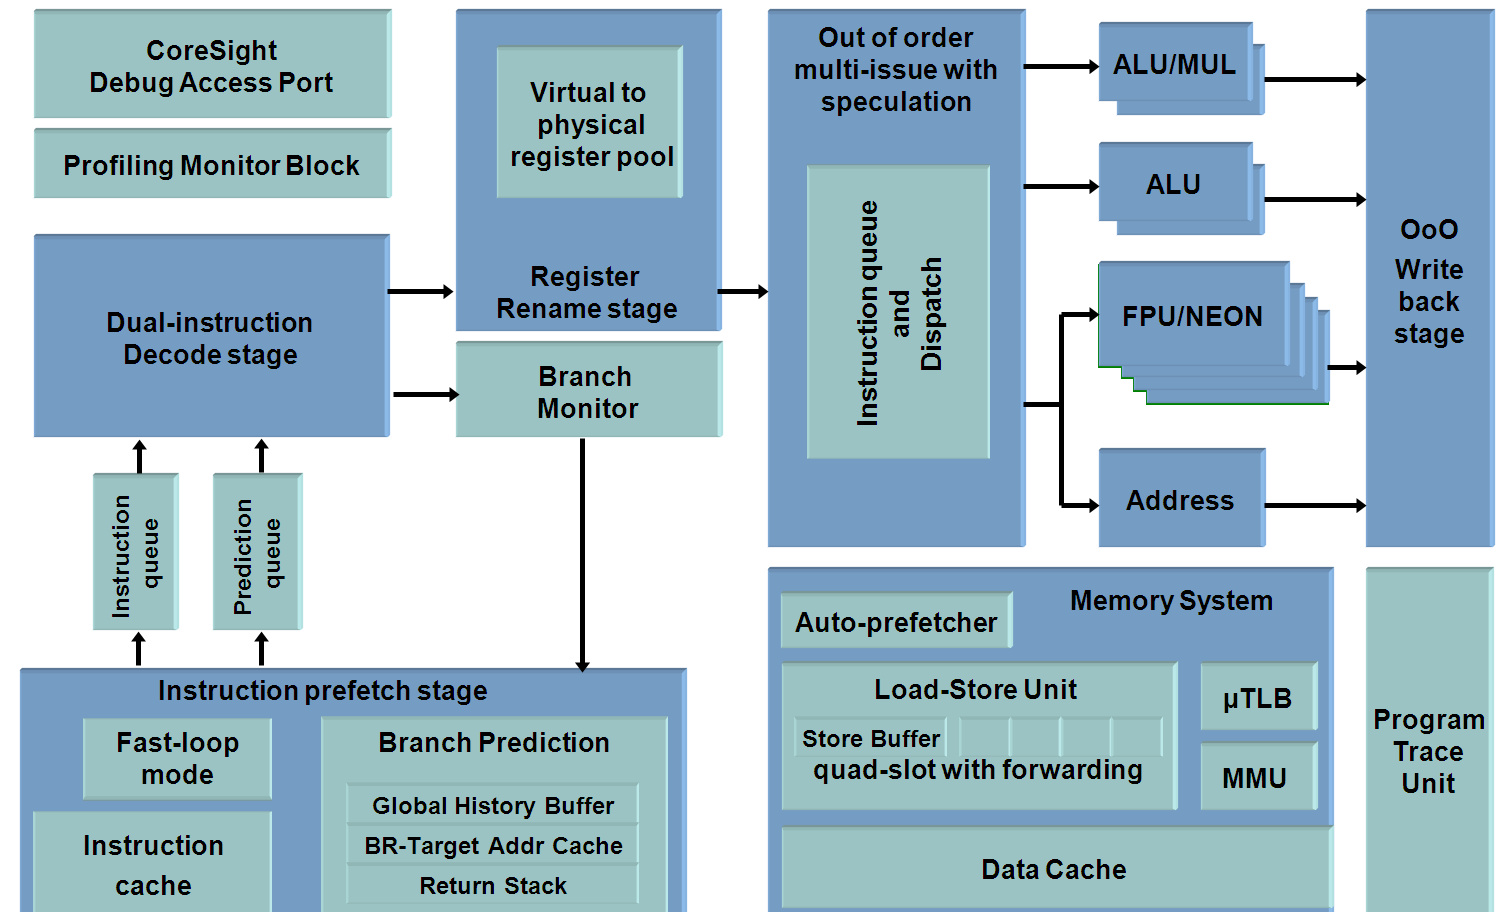
\includegraphics[width=0.48\textwidth]{figures/A9-Pipeline-hres}
        \caption{ARM Cortex-A9 Pipeline and peripherals,\hfill
        figure from ARM Cortex-A9 Whitepaper\cite{a9whitepaper}}
        \label{fig:pipeline}
    \end{centering}
\end{figure}

In general, energy consumption of a processor varies with respect to the
workload; the harder it has to work, the more energy it uses. In this paper, we
seek to achieve the highest possible ALU throughput the processor can offer. To
accomplish this, we are required to gain knowledge of its pipeline and other
components within the CPU.

Official documentation of the pipeline structure is limited to the ``Cortex-A9
Technical Reference Manual'' \cite{armtech} and ``The ARM Cortex-A9 Processors''
whitepaper \cite{a9whitepaper}. However, by running some architectural
experiments and consulting the performance counters we are able to
infer some details.

\subsection{Architectural Experiments}
\label{arch_experiments}
The A9 processor has 58 distinct events\footnote{A complete overview can be seen
in table A.18 in the Cortex-A9 Technical Reference Manual \cite{armtech}} that
each can be mapped to one of six generic event counters in the Performance
Monitor Unit (i.e. only six generic events can be tracked simultaneously). It
also has a separate cycle counter. By comparing execution unit counters for the
two ALUs and the cycle counter, we obtain detailed statistics about the
pipeline activity. For example, we run \texttt{add} instructions with and
without hazards, and verify that counters for the hazard-less run completes
twice in about half the number of cycles. Note that these performance counters are
approximate due to speculativity in the core, and is only being used as a sanity
check for what we expected.

Using performance counters as above, we are able to confirm a feature on the A9
processor that is very vaguely documented; fast-loop\texttrademark{} mode. As
the name suggests, this feature enables rapid execution of small loops. It does
so by fetching instructions from the icache only at the first loop iteration,
effectively voiding time and energy spent on instruction cache lookups between
iterations. However, which loops that falls into this category is not
documented, but by using performance counters we are able to determine this with
confidence. We disable the L1 cache, penalizing runs that do not fit into
fast-loop, making it easy to distinguish between runs within and outside
fast-loop. We find that for loops to be executed in fast-loop it must keep two
premises. First, the loop body must have 15 instructions or less. Secondly, it
must be aligned to a 64 byte cache line, i.e. the first instruction in the loop
must be on a 64-byte aligned address. Violating any of these two properties
will cause code to be executed outside fast-loop and yield a significant
decrease in performance.

Furthermore, executing code within fast-loop limits the number of cache
miss predicts to two independent of the iteration count. We confirm this by
looking at the cache miss predict performance counter. The first miss is likely to
occur at the end of the first iteration, while the second occurs on the way out
of the loop.

\subsection{Benchmarks}
As a first approximation, the benchmark programs consists of an infinite series
of identical instructions. The A9 core runs at a fixed frequency and we are
providing a fixed core voltage, so energy usage (in Watts) for a one-cycle
instruction is determined by the following formula.

\begin{equation}
    P_{instruction} = A_{instruction} \cdot V_{core}
    \label{eq:1}
\end{equation}

Running for a fixed time period, we obtain an expression for the energy used.

\begin{equation}
    E_{instruction} = P_{instruction} \cdot cycles
    \label{eq:2}
\end{equation}

This simple setup does not take the memory system into account; we are
undoubtedly not able to feed the processor instructions at no cost in terms of
access speed and -- more importantly -- memory system energy usage. Thus, we
enhance our setup by running all benchmark code within fast-loop. To explicitly
feed the processor instructions without the overhead of interupts, we write
Linux kernel modules that once inserted, execute a loop similar to the one shown
in \autoref{list:inst_loop}. Note that the \texttt{subs} and \texttt{jne}
instructions are needed to avoid memory fetches completely, but also makes the
program terminate -- which again eases the testing procedure.

The technical manual states that branching to immediate locations
does not consume execution unit cycles. Our microbenchmarks branches to
immediate locations, but it does so conditionally. We assume that the
calculation of this condition takes normal execution time, but that the branch
is invisible.

\begin{figure}
    \begin{lstlisting}{language=[ARM]Assembler}
    label:
    instruction
    ... ; repeats 13X
    instruction
    subs
    jne label
    \end{lstlisting}
    \caption{Instruction loop}
    \label{list:inst_loop}
\end{figure}

\subsection{Power Measurements}
To measure energy consumption, we use an Agilent 34410A
multimeter\cite{agilent34410a} to sense the voltage drop over a negligible
12m$\Omega$ resistor, set up as shown in \autoref{fig:setup}. The multimeter is
configured to sample at full precision at its maximum rate of 1000 Hz. This
gives one sample every 1.7 million instructions with an error of at most 0.002V.
It is obvious that we are unable to observe inter-cycle fluctations with this
equipment, but as we run the same instruction practically indefinetely we get an
average. The instruction loop runs for about 20 seconds for each instruction and
we use 5 seconds in the middle of this period to gather 5000 samples.

Observational errors are accounted for by running the power measurement loop
many times for each instruction. We also sleep 30 seconds in between
instructions to diminish the effect of temperature variations. Running over all
tested instructions typically takes 3 hours and we average the medians for each
instruction run to get a single value.

We separate power consumption on the ARM cores and the development board by
modifying the ODROID-X2 and providing a separate power supply for the A9 cores.
They get powered by an external power supply giving $1.3V$ DC, while the rest of
the board is powered from a another power supply at $5.0V$, as depicted in
\autoref{fig:setup}.

Some instructions takes a different amount of time, the power drain has to
be normalized using statistics gained from performance counters. An instruction
that occupies the pipeline for two cycles, is believed to use approximately
twice as much energy. By normalizing, we can convert point-in-time energy
consumption in terms of Watts to energy per instruction (in Joules).


\subsection{Pitfalls}
% temperature, noise (inducted power, etc.), interrupts, memory latency
% (fast-loop)
We are comparing the energy efficiency of different instructions in an
asynchronous way, so we try to fixate as many parameters as possible. We must
acknowledge that some factors affects power consumption and produces noise in
our data.

\label{sec:temperature}
One obvious such factor is the chip temperature: it is known that power
consumption increases at higher core temperatures. We explore the boundaries by
physically applying freeze spray and notice that our measurements gets 4\%
higher with a temperature increase from 9 to 63 Celsius. The \texttt{mul}
instruction had the greatest leap and used 7\% more energy at 63 degrees. In our
experiments, only one of the four available cores are used. Stressing a single
core over time did not increase temperature by more than 7 degrees (from idle at
47$^\circ$ C to 54$^\circ$ C at load), so the chip is evidently able to
dissipate more heat than one core can generate. Assuming that it is generally
true that a single core cannot heat the entire SoC significantly,
and that the increase in power consumption is at most 10\% over 50$^\circ$
Celsius, we get

\begin{equation}
    P_{inc} = P_{orig} \cdot T_{inc} \cdot \frac{0.10}{50} = P_{orig} \cdot T_{inc} \cdot 0.002
\end{equation}

Believing that this trend is at least close to linear, output will increase by
0.2\% pr. degree Celsius increased. Also, we start our measurements several
seconds after the benchmarks itself starts, giving the core plenty of time to
gain work temperature. In our tests, the time used to get to work temperature
was humanly instant. Note that we could not log temperature from on-chip sensors
while running our tests, as these sensors are tightly coupled with DVFS in the
Linux kernel, which we have disabled.

Another factor that is not that obvious, but equally important, is power
induced in the measurement circuit. Since wires are often winded up on the test
bench, and lab equipment might contain large metal cores with a great amount of
power running through them, unexpected power might be introduced.

Running Linux as the base environment for our tests gives us a much simpler
abstractions to make the processor run our programs, but it also comes with some
caveats. Having an entire operating system beneath our benchmark programs
implies that there is much going on that we have no direct controls over. In
order to mitigate the artifacts originating from the operating system, we
disable all the maskable interrupts and run our benchmark programs entirely
uninterupted.

As explained in section \ref{arch_experiments}, we utilize the fast-loop mode of
the processor to mitigate memory access latency. We disable the L1 cache to
easier detect when we are outside the fast-loop mode, and thus we are certain
that there is no memory access going on.
